\section{EXPERIMENTAL RESULTS}
\label{sec:exp}


This section presents the results of using our implementation (Algorithm~\ref{multimon}) for reducing
circuits used in cryptography. We compare our results against F4-style reduction~\cite{pruss:tcad}, 
parallelized approach for performing reductions on Galois field multipliers~\cite{cunxi:aspdac17}, 
and PolyBori~\cite{polybori:2009} that uses the conventional reduction procedure on top of ZBDDs. 
The experiments are performed on a 3.5GHz Intel 
Core\textsuperscript{TM} i7-4770K Quad-Core CPU with 32 GB of RAM. 
% Modular multiplication is an important computation used in cryptography. 
% We have performed experiments with two architectures for this multiplication, namely Mastrovito and Montgomery. 

\subsection{Mastrovito Multipliers}

Modular multiplication is an important computation used in cryptography. 
A Mastrovito multiplier architecture can be employed for performing this computation.
Mastrovito multipliers compute $Z = A\times B \pmod{
  P(x)}$ where $P(x)$ is a given primitive polynomial for the datapath size
$k$. 

The product $A \times B$ is computed using an array multiplier architecture, and then the result is reduced modulo $P(x)$.
The following example demonstrates the Mastrovito multiplier computation~\cite{lv:tcad2013}.
%take $\{A,B\} =
%\{a_0,a_1,\dots,a_{k-1},b_0,b_1,\dots,b_{k-1}\}$ as $k$-bit inputs and
%produce $Z = \{z_0,z_1,\dots,z_{k-1}\}$ as $k$-bit output. The multiplier
%performs $Z = A \times B \pmod{P}$, 

%The procedure 
%involves computing the product $S=A\times B$ using an array multiplier
%and then reducing it $\pmod{P}$ to obtain $Z$. We perform experiments
%on \textit{flattened} netlists of these circuits.  

\begin{Example}
\label{exp1}
{\it 
Consider the field $\mathbb{F}_{2^4}$. Let the inputs be:
$A=a_0+a_1\cdot \alpha+a_2\cdot \alpha^2+a_3\cdot \alpha^3$ and
$B=b_0+b_1\cdot \alpha+b_2\cdot \alpha^2+b_3\cdot \alpha^3$, and 
 the irreducible polynomial be $P(x)=x^4+x^3+1$. 
 % We have to perform the multiplication $Z =A\times B \pmod{ P(x) }$. 
 The coefficients of $A = \{a_0, \dots, a_3\}, B = \{b_0, \dots, b_3\}$ are in
$\mathbb{F}_2 = \{0, 1\}$. First, we perform the multiplication as:

%\vspace{-0.2in}

\vspace{0.05in}

{\small
{\begin{tabular}{c c c c c c c c}
%\vspace{-0.2in}
  &   &   & $a_3$ & $a_2$ & $a_1$ & $a_0$  \\ 
 $\times$&   &   & $b_3$ & $b_2$ & $b_1$ & $b_0$  \\ 
 \hline
 &   &   & $a_3\cdot b_0$ & $a_2 \cdot b_0$ & $a_1\cdot b_0$ & $a_0\cdot b_0$ \\
 &  & $a_3\cdot b_1$ & $a_2\cdot b_1$ & $a_1 \cdot b_1$ & $a_0\cdot b_1$ &   \\
 & $a_3\cdot b_2$ & $a_2\cdot b_2$ & $a_1\cdot b_2$ & $a_0\cdot b_2$ &  &   \\
 $a_3\cdot b_3$ & $a_2\cdot b_3$ & $a_1\cdot b_3$ & $a_0\cdot b_3$ &  &  &   \\
 \hline
 $s_6$& $s_5$  & $s_4$  & $s_3$ & $s_2$  & $s_1$   & $s_0$ 
% \vspace{-0.2in}
\end{tabular}}
}

\vspace{0.05in}

The result $Sum = s_0+s_1\cdot \alpha + s_2\cdot \alpha^2 + s_3\cdot
\alpha^3 + s_4\cdot \alpha^4 + s_5\cdot \alpha^5 + s_6\cdot \alpha^6$,
where, $s_0  =  a_0\cdot b_0, ~~s_1  =  a_0\cdot b_1 + a_1\cdot b_0,
~~s_2 = a_0\cdot b_2 + a_1\cdot b_1 + a_2\cdot b_0$, and so on. Here
the multiply ``$\cdot$'' and add ``$+$'' operations are performed
modulo 2, and hence implemented in a circuit using AND and XOR
gates. As the coefficients are always reduced modulo $p =
2$, there are no carry-chains
in the design. Next, the result is reduced modulo the primitive
polynomial $P(x) = x^4 + x^3 + 1$, as:
% where the final output of the circuit is denoted by $G(x)  = g_3x^3
% + g_2x^2 +g_1x + g_0$.  

\vspace{0.05in}

{\small
{\begin{tabular}{|c c c c | l }
  $s_3$   &$s_2$    &$s_1$   &$s_0$   &   \\
 \hline
 $s_4$    &$0$    &$0$   &$s_4$   &$s_4\cdot \alpha^4 \pmod{P(\alpha)} = s_4 \cdot (\alpha^3 + 1)$\\
 $s_5$    &$0$    &$s_5$   &$s_5$     &$s_5\cdot \alpha^5 \pmod{P(\alpha)} = s_5\cdot (\alpha^3+ \alpha + 1)$\\
 $s_6$    &$s_6$    &$s_6$   &$s_6$     &$s_6\cdot \alpha^6 \pmod{ P(\alpha)} = s_6\cdot( \alpha^3 + \alpha^2 + \alpha + 1)$\\
 \hline
 $z_3$    &$z_2$    &$z_1$   &$z_0$   &
 \end{tabular}\par}
}

\vspace{0.05in}

The final output of the circuit is: $Z = z_0 + z_1 \alpha + z_2
\alpha^2 + z_3 \alpha^3$; where  $z_0=s_0+s_4+s_5+s_6; ~~z_1=s_1+s_5+s_6;
~~z_2=s_2+s_6; ~~z_3=s_3+s_4+s_5+s_6$. 
}
\end{Example}

\par Table~\ref{masmmsyn} provides the results for the reductions $z_i \xrightarrow{G}_+ r_i$ for Mastrovito multipliers for each output bit $z_i$.
The benchmarks are taken from~\cite{lv:tcad2013} which are optimized using ABC~\cite{ABCtool} with the same commands and library as mentioned in~\cite{cunxi:aspdac17}. Algorithm~\ref{multimon} reduces each output bit independent of other bits. Therefore, we have presented the results obtained by running our reduction algorithm both parallely and sequentially for each output bit. Similarly, the results for implementation in PolyBori are also presented for both cases. The maximum number of parallel processes is decided by the memory usage of each process ($i.e.$ reducing one bit) for our implementation and the total available memory. The larger benchmarks are run with fewer parallel processes as they consume more memory ($e.g.$ 64-bit 
benchmark is run with 20 processes where 409-bit with only 10). 

% For example,in Table~\ref{masmmsyn}, the 64 bit multiplier is run with 20 
% threads, whereas 571 bit with only 3.

% As ZBDDs are more complex data structures compared to those used in~\cite{cunxi:aspdac17}, the upper limit of memory usage for each bit is set by our implementation. For instance, an individual process in the reduction of 283-bit multiplier can take upto $\sim 3\%$ of available memory as compared to $\sim 6\%$ in the case of 409-bit mulitplier. Therefore, we run the all the implementations with 20 parallel processes for 283-bit multiplier but only with 10 for 409-bit multiplier. 
\par In the table, the column \#T represents the number of parallel processes. (S) and (P) refer to the cases when the experiments are run sequentially and parallely for the output bits $z_i$, respectively. 

%%%%%%%%%%%%% Syn Mas Multipliers %%%%%%%%%%%%%%%%%%%
%\iffalse
\begin{table}[H]
\centering
%\caption{Synthesized Mastrovito Multipliers (Time in seconds, \# of nodes, \# of redundant monomials in $k$)  (K = $10^3$, M = $10^6$)}
\caption{Mastrovito Multipliers (Time in seconds);  k = Datapath Size, \#Gates = No. of gates, \#T = No. of threads, Time-Out = 30 hrs, (P): Parallel Execution, (S): Sequential Execution, K = $10^3$, M = $10^6$, PB: PolyBori, ZR: Algorithm~\ref{multimon}}
\label{masmmsyn}
\begin{tabular}{| c | c | c | c | c | c | c | c | c |} \hline
%\multirow{2}{*}{\textbf{Input}} & \multirow{2}{*}{\textbf{Abstraction}} & \multicolumn{3}{ c |}{\textbf{ZBDD reduction(ZR)}}  &  \multirow{2}{*}{\textbf{ZR improved}}\\ \cline{3-5}
% & &Building ZBDDs&Reduction&Total&\\ \hline
\multirow{2}{*}{\textbf{k}}&\multirow{2}{*}{\textbf{\#Gates}}&\multirow{2}{*}{\textbf{F4~\cite{pruss:tcad}}}& \multirow{2}{*}{\textbf{\#T}}&\multirow{2}{*}{\textbf{~\cite{cunxi:aspdac17}(P)}}& \multicolumn{2}{ c |}{\textbf{PB}}&\multicolumn{2}{ c |}{\textbf{ZR}}\\ \cline{6-9}
&&&&&\textbf{(P)}&\textbf{(S)}&\textbf{(P)}&\textbf{(S)} \\ \hline
64 &11.5K&1.3&20& 3.70&3.60& 2.21&0.73 &\textbf{0.27}\\ \hline 
% 96 &25.6K&&20& 11.66&10.25&6.92 &2.04 &\textbf{0.66}\\ \hline 
128 &46K&9.89&20&27.54 &23.99&16.76& 5.08 &\textbf{1.63}\\ \hline 
163 &73.5K&32.61&20& 55.96&48.67&33.72&  11.41&\textbf{3.11}\\ \hline 
233 &122K&86.30& 20&127.61&112.96 &77.23& 21.77&\textbf{3.63}\\ \hline
283 &193K&274.68& 20&253.05&227.77&157.45& 49.89&\textbf{11.41}\\ \hline
409 &386K&2,528.48& 10&716.80 &659.64&426.92& 163.52&\textbf{17.68}\\ \hline
571* &1.6M & TO &3 & 5,331&CR&CR&2,126.65& \textbf{566.39}\\ \hline
\end{tabular}
\end{table}
%\fi

%%%%%%%%%%%%%%%%%%%%%%%%%%%%%%%%%%%%%%%%%
\par The 571-bit multiplier could not be synthesized and mapped with the given memory. Therefore, we have provided results for a structured (but not optimized) 571-bit multiplier benchmark. Our implementation outperforms the explicit approaches of~\cite{pruss:tcad} and~\cite{cunxi:aspdac17} for Mastrovito multipliers. For the 571-bit multiplier, the implementation of~\cite{pruss:tcad} does not finish for the given time period of 30 hours and the PolyBori implementation crashes (CR).

\par An interesting point to note in the Table~\ref{masmmsyn} is that our implementation takes less time when we are running it sequentially. There is a certain overhead involved when we declare variables and build ZBDDs for each gate of the circuit. In the case of Mastrovito multipliers benchmarks, this overhead is substantially greater than the actual reduction time for each output bit. Consequently, when we run these benchmarks parallely this overhead time hampers the overall run time. Therefore, parallelization only improves the run time when the overhead time is smaller than the actual reduction time. 
% For example, for the 64-bit multiplier the overhead is 22.09 ms (when running it sequentially), whereas the reduction time for most of the bits is $\sim 0.30$ ms. The sequential reduction time with these values is $22.09 + 64 (0.3) = 41.29$ ms. On the other hand, with 20 processes this time is approximately $(64/20)(22.09 + 0.3) = 71.65$ ms. 
% There are other factors involved too, $e.g.$ CUDD package maintains an internal cache that helps avoid duplicate computations. When performing reduction sequentially the operations involving fanouts can be stored in the cache and used during the reduction of different output bits. 
% \vspace{-0.1in}
\subsection{Montgomery Multipliers}
Exponentiation (repeated multiplication) is often required in cryptosystems.  
For such applications, Montgomery architecture \cite{acar:1998} \cite{wu:2002}
% \cite{Barrett:1987} 
\cite{Knezevic:2008} are considered more efficient than Mastrovito multipliers
as they do not require explicit reduction modulo $P(x)$ after each step.
% Montgomery multipliers perform fast modular multiplication without
% explicitly performing the reduction $\pmod{P}$. 
%They are more
%efficient than the Mastrovito multipliers when several modulo
%multiplications are required as in the case of exponentiation in
%cryptosystems. 
Fig.~\ref{montfig} shows the structure of a Montgomery
multiplier. Each MR block computes $A\cdot B\cdot R^{-1}$, where $R$
is selected as a power of a base ($\alpha^{k}$) and $R^{-1}$ is the multiplicative 
inverse of $R$ in $\mathbb{F}_{2^k}$. As this operation cannot compute $A\cdot B$
directly, we need to pre-compute $A\cdot R$ and $B\cdot R$ as shown in the Fig.~\ref{montfig}. 
We denote the leftmost
two blocks as Block A (upper) and B (lower), the middle block as Block
C and the output block as Block D.
% We have presented results for GBR
%on both \textit{flattened} and \textit{hierarchical} netlists of these
% multipliers. 

\begin{figure}[H]
  \centering
  %\def\svgwidth{340pt}
  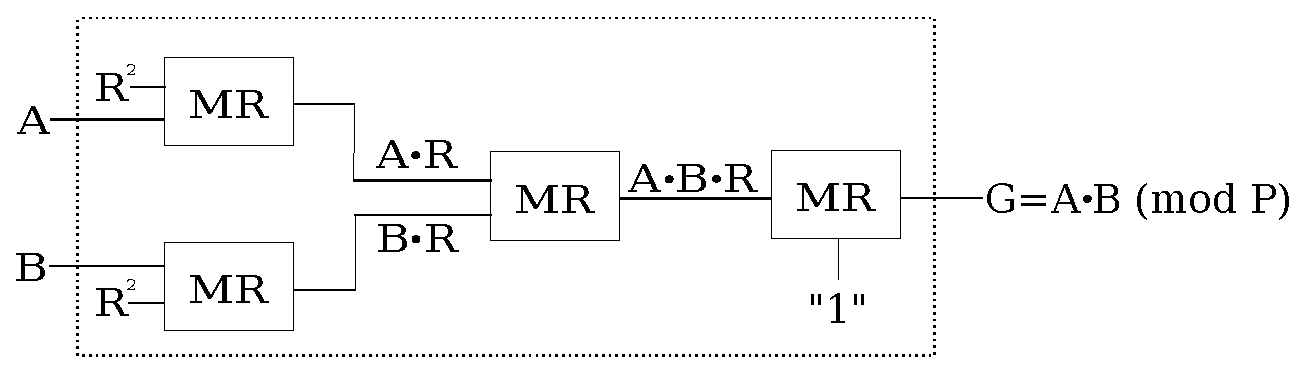
\includegraphics[scale=0.34]{new_mmcircuit}
  \caption{Montgomery multiplication.}
  \label{montfig}
  \end{figure}
\vspace{-0.1in}
\par Table~\ref{montmmsyn} provides the results for flattened (bit-blasted) and optimized Montgomery multipliers for the sequential and parallel executions. 
% For most of these benchmarks the overhead is quite small than the reduction time for one bit except for the 233 and 409 bit multipliers. Therefore, we benefit from parallelizing the reduction process for these cases other than 283 and 409 bit multipliers. 
The 571-bit benchmark in the table is an unoptimized structured benchmark. We again get a significant improvement over the explicit approaches except for the case of 283 bit multiplier. 


%%%%%%%%%%%%% Syn Mont Multipliers %%%%%%%%%%%%%%%%%%
%\iffalse
\begin{table}[H]
\centering
%\caption{Synthesized Mastrovito Multipliers (Time in seconds, \# of nodes, \# of redundant monomials in $k$)  (K = $10^3$, M = $10^6$)}
\caption{Montgomery Multipliers (Time in seconds); k = Datapath Size, \#Gates = No. of gates, \#T = No. of threads, Time-Out = 30 hrs, (P): Parallel Execution, (S): Sequential Execution, K = $10^3$, M = $10^6$, PB: PolyBori, ZR: Algorithm~\ref{multimon}}
\label{montmmsyn}
\begin{tabular}{| c | c | c | c | c | c | c | c | c |} \hline
%\multirow{2}{*}{\textbf{Input}} & \multirow{2}{*}{\textbf{Abstraction}} & \multicolumn{3}{ c |}{\textbf{ZBDD reduction(ZR)}}  &  \multirow{2}{*}{\textbf{ZR improved}}\\ \cline{3-5}
% & &Building ZBDDs&Reduction&Total&\\ \hline
\multirow{2}{*}{\textbf{k}}&\multirow{2}{*}{\textbf{\#Gates}}&\multirow{2}{*}{\textbf{F4~\cite{pruss:tcad}}}& \multirow{2}{*}{\textbf{\#T}}&\multirow{2}{*}{\textbf{~\cite{cunxi:aspdac17}(P)}}& \multicolumn{2}{ c |}{\textbf{PB}}&\multicolumn{2}{ c |}{\textbf{ZR}}\\ \cline{6-9}
&&&&&\textbf{(P)}&\textbf{(S)}&\textbf{(P)}&\textbf{(S)} \\ \hline
64 &9.5K&16.29&20&10.69&6.27&9.22& \textbf{3.75} & 8.37\\ \hline 
%96 &20.3K&&20&36.40&24.22& 22.0&\textbf{17.56} & 21.15\\ \hline 
128 &35K&621.90&20& 36.19&28.93&34.59&  \textbf{13.76}&24.73\\ \hline 
163 &56.5K&2,608.4&20&204.94 &167.73&335.24&  \textbf{141.68}&321.60\\ \hline 
233 &111K&385.92& 20&132.51& 119.77&99.36 &42.16&\textbf{31.88}\\ \hline
283 &165K&5,344& 20&\textbf{704.13}&1,194.2&2,078.1& 1,065.3&2,113.0\\ \hline
409 &340K&7,104& 10& 697.91&737.23& 722.05&303.91&\textbf{299.92}\\ \hline
571* &1.97M&TO&3&TO&CR&CR&\textbf{43,813}&99,042 \\ \hline
\end{tabular}
\end{table}
%\fi
%%%%%%%%%%%%%%%%%%%%%%%%%%%%%%%%%%%%%%%%%

\par Table \ref{montblockmm} presents the
statistics for hierarchical Montgomery multipliers for the blocks A,
B, C, and D. The experiment first reduces the outputs of a block
modulo the gates of that block, and then reduces the primary outputs
modulo these four sets of remainders (ZBDDs), thus exploiting the
hierarchy of these circuits. Table~\ref{montblockmm} shows the time
for reduction of each block and the time for reducing the primary
outputs across the four levels. The  time for reducing the primary
outputs across  levels in case of F4 implementation is $<$1 second,
and is not explicitly mentioned in the table. The row labeled
\textit{Total} presents the sum of time of reduction across levels and
the maximum reduction time for each block (as the reductions for the
four levels are and done independent of each other). 
% The datapath sizes of these circuits correspond to
% NIST-specification in cryptography with $k = 163,\dots,571$ bits.

\begin{table}[H]
\centering
% \caption{Montgomery Blocks(Time in seconds, Red. = time for reduction,
%   Coll. = time to reduce across the 4 levels.)}
\caption{Montgomery Blocks (Time in seconds); k = Datapath Size, \#Gates = No. of gates, Time-Out = 30 hrs, 
Red. = time for reduction, Coll. = time to reduce across the 4 levels. 
% (P): Parallel Execution, (S): Sequential Execution, 
K = $10^3$, M = $10^6$, PB: PolyBori, ZR: Algorithm~\ref{multimon}}

\label{montblockmm}
\begin{tabular}{| c | c | c | c | c | c | c | c |} \hline
\multirow{2}{*}{\textbf{k}}& \multirow{2}{*}{\textbf{\#Gates}}&\multirow{2}{*}{\textbf{Block}}& \multirow{2}{*}{\textbf{F4~\cite{pruss:tcad}}}  & \multicolumn{2}{ c |}{\textbf{PB}} &  \multicolumn{2}{ c |}{\textbf{ZR}} \\ \cline{5-8}
  & & & &Red. & Coll.  &Red. & Coll.  \\ \hline
\multirow{4}{*}{163} &33K &Block A & 25& 12 &\multirow{4}{*}{16} & 1 & \multirow{4}{*}{18}\\  \cline{2-5} \cline{7-7}
 & 33K&Block B &25 & 12 & & 1  &  \\  \cline{2-5} \cline{7-7}
 &85K&Block C &73 & 18 &&  7 &  \\  \cline{2-5} \cline{7-7}
 &32K&Block D &24 & 12 & & 1 & \\ \cline{2-8}
 &\multicolumn{2}{ c |}{\textbf{Total}} & 73  &   \multicolumn{2}{ c |}{34} & \multicolumn{2}{ c |}{\textbf{25}}\\ \noalign{\hrule height 1.5pt}
\multirow{4}{*}{233}&55K&Block A  &142  & 32 & \multirow{4}{*}{5} & 0.14 & \multirow{4}{*}{4}\\  \cline{2-5} \cline{7-7}
 &55K& Block B &141 & 33 && 0.14  &  \\  \cline{2-5} \cline{7-7}
 &163K&Block C &408 & 34 & & 2.1  &  \\  \cline{2-5} \cline{7-7}
 &54K&Block D & 140& 32 && 0.13 & \\ \cline{2-8}
&\multicolumn{2}{ c |}{\textbf{Total}}& 408  &   \multicolumn{2}{ c |}{39} & \multicolumn{2}{ c |}{\textbf{6.1}}\\ \noalign{\hrule height 1.5pt}
\multirow{4}{*}{283}&82K&Block A & 330 & 79 & \multirow{4}{*}{26} &24 & \multirow{4}{*}{90}\\  \cline{2-5} \cline{7-7}
&82K & Block B &329 & 78 && 23  &  \\  \cline{2-5} \cline{7-7}
&241K &Block C &883 & 173 &&  118 &  \\  \cline{2-5} \cline{7-7}
&81K &Block D &321 & 80 && 23 & \\ \cline{2-8}
&\multicolumn{2}{ c |}{\textbf{Total}} & 883  &   \multicolumn{2}{ c |}{\textbf{199}} & \multicolumn{2}{ c |}{208}\\ \noalign{\hrule height 1.5pt}
\multirow{4}{*}{409}&168K&Block A & 1,322 & 177&\multirow{4}{*}{28} & 0.57 & \multirow{4}{*}{29}\\ \cline{2-5} \cline{7-7}
& 168K& Block B &1,335 &  175 &&  0.57 &  \\ \cline{2-5} \cline{7-7}
& 502K&Block C &4,471 & 192 &&  14 &  \\  \cline{2-5} \cline{7-7}
&168K &Block D &1,338 & 176 && 0.56 & \\ \cline{2-8}
&\multicolumn{2}{ c |}{\textbf{Total}} & 4,471  &   \multicolumn{2}{ c |}{220} & \multicolumn{2}{ c |}{\textbf{43}}\\ \noalign{\hrule height 1.5pt}
\multirow{4}{*}{571}&330K&Block A &5,371 & 769 & \multirow{4}{*}{1,341} &321  & \multirow{4}{*}{1,412}\\  \cline{2-5} \cline{7-7}
&330K & Block B &5,421 & 747 && 332  &  \\ \cline{2-5} \cline{7-7}
 &980K&Block C &37,804 & 3,605 &&  3026 &  \\  \cline{2-5} \cline{7-7}
 &328K&Block D &5,539 & 751 && 338 & \\ \cline{2-8}
&\multicolumn{2}{ c |}{\textbf{Total}}& 37,804  &   \multicolumn{2}{ c |}{4,946} & \multicolumn{2}{ c |}{\textbf{4,438}}\\ \noalign{\hrule height 1.5pt}


\end{tabular}
\end{table}
% \vspace{-0.1in}
 %%%%%%%%% Point Addition Block D%%%%%%%%%%%%%%%%%%%%%%%%
\subsection{Point Addition over Elliptic Curves}
Point addition is an important operation required for the task of encryption, decryption 
and authentication in Elliptic Curve Cryptography (ECC). 
Modern approaches represent the points in a projective
coordinate systems, {\it e.g.}, the L$\acute{o}$pez-Dahab (LD) projective coordinate \cite{eccld} due to which the point addition 
operation can be implemented as polynomials in the field. 

\begin{Example}
{\it Consider point addition in L$\acute{o}$pez-Dahab (LD) projective coordinate. Given an elliptic curve: $Y^2 + XYZ = X^3Z + aX^2Z^2 + bZ^4$ over $\mathbb{F}_{2^k}$, where $X,Y,Z$ are $k$-bit vectors that are elements in $\mathbb{F}_{2^k}$ and similarly, $a, b$ are constants from the field. We represent point addition over the elliptic curve as ($X_3$, $Y_3$, $Z_3$) = ($X_1$, $Y_1$, $Z_1$) + ($X_2$, $Y_2$, $1$).  Then $X_3$, $Y_3$, $Z_3$ can be computed as follows:} 

\begin{align*}
&A = Y_2 \cdot Z_1^2 + Y_1  &&B = X_2 \cdot Z_1 + X_1 \\
&C = Z_1 \cdot B  &&D = B^2 \cdot(C + a Z_1^2) \\
&Z_3 = C^2 && E = A \cdot C  \\
&X_3 = A^2 + D + E &&F = X_3 + X_2 \cdot Z_3 \\
&G = X_3 + Y_2\cdot Z_3 && Y_3 = E\cdot F + Z_3 \cdot G \\
\end{align*}
\end{Example}

\begin{table}[H]
\centering
\caption{Point Addition Circuits (Time in seconds); k = Datapath Size, \#Gates = No. of gates, K = $10^3$, M = $10^6$}
\label{pointadd}
\begin{tabular}{| c | c | c | c | c |} \hline
\textbf{k}&\textbf{\#Gates}&\textbf{F4~\cite{pruss:tcad}}&\textbf{PB}&\textbf{ZR} \\ \hline
64&15.3K&1.78&3.32&\textbf{0.72} \\ \hline
128&64K&40.55&27.41&\textbf{6.03} \\ \hline
163&104K&130.24&57.57&\textbf{13.13} \\ \hline
233&139K&335.60&106.85&\textbf{19.62} \\ \hline
283&281K&1,787.96&273.53& \textbf{64.48}\\ \hline
409&423K&5,077.50&578.15& \textbf{115.20}\\ \hline
571&1.14M&48,162.29&CR&\textbf{725.95} \\ \hline
\end{tabular}
\end{table}

The word-level abstraction approach in~\cite{pruss:tcad} presents the results for extracting 
the above representation for each of $A,B,\dots, X_3,Y_3,Z_3$. It first performs a bit-level reduction and then a 
bit to word substitution for the primary input bit variables. Table~\ref{pointadd} shows 
the comparison of the bit-level reduction of ECC Point addition circuits as done in~\cite{pruss:tcad}
against our implementation. 
% This bit level reduction is for the intermediate 
% computation of $D$ that takes longest time for the implementation in~\cite{pruss:tcad}. 
This result demonstrates that our implementation can be integrated with that of~\cite{pruss:tcad} to improve the overall process.  
\par {\bf Integer Multiplication:} When performing reduction on integer multiplication benchmarks, a large number of non-linear 
monomials are generated that can be canceled early in the reduction process by employing a word-level approach unlike 
our bit-level reduction approach.


%%%%%%%%%%%%%%%%%%%%%%%%%%%%%%%%%%%%%%%%%%%%%%%%%%%%%%%%

\section{Conclusion}
This paper has presented an approach to derive a canonical polynomial
representation for each output bit $z_i$ of a circuit, by modeling the gates
of the circuit as a set of polynomials $G$ over $\mathbb{F}_2$, and
performing the reduction $z_i\xrightarrow{G}_+ r_i$. 
%The complexity of computing the
%Gr\"obner basis can be avoided by deriving a term order from the
%topology of the circuit, which renders this set of polynomials itself
%as  a Gr\"obner basis. 
The unate cube set algebra prowess of ZBDDs is exploited to represent
the polynomials implicitly. We take further advantage of this
data structure to improve the classical \Grobner basis reduction
method that relies on canceling only 1 monomial in every iteration
of division. Our approach cancels multiple monomials in each step of
division, thus speeding up the reduction. 
The  efficiency of our approach is demonstrated by completing  the
reduction for up to 571-bit modulo multipliers in the allotted time,
and significant improvement is achieved over the F4-style reduction,
parallelized reductions and  PolyBori based techniques. As part of our future work, we will be
pursuing word-level implementation of the polynomial reduction
for integer arithmetic circuits.  
\par \textbf{Acknowledgement:} The authors wish to thank Cunxi Yu for 
assistance with optimization of the
benchmarks used in the experiments. 
%\end{document} 
%%%%%%%%% Mas571 Multipliers %%%%%%%%%%%%%%%%%%%%%%%%
\iffalse
\begin{table}[H]
\centering
\caption{Structured 571 bit Multipliers (Time in seconds);  \#Gates = No. of gates, \#T = No. of threads, Time-Out = 1 day, (P): Parallelization, (WP): Without Parallelization, K = $10^3$}
\label{montmmsyn}
\begin{tabular}{| c | c | c | c | c | c | c | c |} \hline
\textbf{Architecture} & \textbf{\#Gates}&\textbf{F4} & \textbf{\#T} & \textbf{~\cite{cunxi:aspdac17}(P)} & \textbf{PB} & \textbf{ZR(P)} & \textbf{ZR(WP)} \\ \hline
Mastrovito&1,600K&TO&3&5,331&CR&2,126.65&566 \\ \hline
Montgomery&1,970K&TO&3&TO&CR&43,813&TO \\ \hline
\end{tabular}
\end{table}
\fi
%%%%%%%%%%%%%%%%%%%%%%%%%%%%%%%%%%%%%%%%%
%%%%%%%%% OLD TABLES%%%%%%%%%%%%%%%%%%%%%%%%%%
%%%%%%%%%%%%%%%%%%%%%%%%%%%%%%%%%%%%%%%%%
%%%%%%%%%%%%%%%%%%%%%%%%%%%%%%%%%%%%%%%%%
\iffalse
\begin{table*}
\centering
\caption{Mastrovito Multipliers (Time in seconds, \# of nodes, \# of redundant monomials in $k$)  (K = $10^3$, M = $10^6$)}
\label{masmm}
\begin{tabular}{| c | c | c | c | c | c | c |} \hline
%\multirow{2}{*}{\textbf{Input}} & \multirow{2}{*}{\textbf{Abstraction}} & \multicolumn{3}{ c |}{\textbf{ZBDD reduction(ZR)}}  &  \multirow{2}{*}{\textbf{ZR improved}}\\ \cline{3-5}
% & &Building ZBDDs&Reduction&Total&\\ \hline
\textbf{Datapath(k)}&\textbf{\# of Gates} & \textbf{F4} & \textbf{PB} &\textbf{ZR} & \textbf{MN/MR} & \textbf{CS}\\ \hline
163 &153K& 1,443s &70s& \textbf{10s} & 811/765 & 153K\\ \hline 
233 &167K& 1,913s &105s& \textbf{14s} & 772/699& 167K\\ \hline
283 &399K& 11,116s &316s& \textbf{45s} & 1,413/1,402&400K\\ \hline
409 &508K& 17,848s &596s& \textbf{75s} & 1,313/1,227&508K\\ \hline
571 &1.6M& 192,032s &CR& \textbf{616s} & 2,849/2,840&1.6M\\ \hline 


\end{tabular}
\end{table*}
\fi

\iffalse
\begin{table*}
\centering
\caption{Montgomery Flat Multipliers (Time in seconds, \# of nodes in $k$, \# of redundant monomials in $k$) (K = $10^3$, M = $10^6$, B = $10^9$)}
\label{montmm}
\begin{tabular}{| c | c | c | c | c | c | c |} \hline
%\multirow{2}{*}{\textbf{Input Bit-width}} & \multirow{2}{*}{\textbf{Abstraction}} & \multicolumn{3}{ c |}{\textbf{ZBDD reduction(ZR)}}  &  \multirow{2}{*}{\textbf{ZR improved}} \\ \cline{3-5}
% & &Building ZBDDs&Reduction&Total& \\ \hline
\textbf{Datapath(k)}&\textbf{\# of Gates} & \textbf{F4} & \textbf{PB} &\textbf{ZR} & \textbf{MN/MR} & \textbf{CS}\\ \hline
163 & 184K&6,897s &\textbf{9294s}&9,595 & 39.4K/765 & 823M\\ \hline 
233 & 329K&63,805s &1749s&\textbf{1,452s}&4.4K/699 & 186M\\ \hline
283 & 488K&TO &\textbf{127,096s}& 247,837s &117K/1.4K &8.7B\\ \hline
409 & 1.0M&TO & \textbf{19,679s}& 32,226s &9.5K/1.2K &1.4B\\ \hline
571 & 1.97M&TO &CR& \textbf{128,464s}& TO/2.9K & TO\\ \hline 

\end{tabular}
\end{table*}
\fi

\iffalse
\begin{table*}
\centering
\caption{Montgomery Blocks(Max Nodes/Remainder)  (K = $10^3$, M = $10^6$)}
\label{montblockstats}
\begin{tabular}{| c | c | c | c | c | c | c |} \hline
\textbf{Datapath(k)/Block} &&  \textbf{163} & \textbf{233} &\textbf{283} & \textbf{409} & \textbf{571} \\ \hline
\multirow{2}{*}{Block A} &MN/MR&64/9&10/5&155/10&11/5& 296/9\\ \cline{2-7}
& CS&301K & 98K& 2.3M & 345K & 17M\\ \hline
\multirow{2}{*}{Block B} &MN/MR&64/9&10/5&155/10&11/5& 296/9\\ \cline{2-7}
& CS&301K & 98K& 2.3M & 345K & 17M\\ \hline
\multirow{2}{*}{Block C} &MN/MR&3.2K/3.2K&705/701&13K/10K&1.2K/1.2K& 83K/82K\\ \cline{2-7}
& CS&301K & 98K& 2.3M & 345K & 17M\\ \hline
\multirow{2}{*}{Block D} &MN/MR&112/58&12/7&292/147&14/8& 578/291\\ \cline{2-7}
& CS&301K & 98K& 2.3M & 345K & 17M\\ \hline
\multirow{2}{*}{Collapse} &MN/MR&18K/765&1.5K/699&42K/1.4K&3K/1.2K& 167K/2.8K\\ \cline{2-7}
& CS& 1.8M& 321K & 12M&1.3M &96M \\ \hline
\end{tabular}
\end{table*}
\fi
%&&&&&&&&&& \\ \hline
%%%%%%%%%%%%%%%%%%%%%%%%%%%%%%%%%%%%%%%%%
%%%%%%%%%OLD TABLES END%%%%%%%%%%%%%%%%%%%%%%%%
%%%%%%%%%%%%%%%%%%%%%%%%%%%%%%%%%%%%%%%%%
%%%%%%%%%%%%%%%%%%%%%%%%%%%%%%%%%%%%%%%%%




\iffalse
\begin{table}
\centering
\caption{Integer Array Multipliers (Time in seconds)}
\label{intmm}
\begin{tabular}{| c | c | c | c | c |} \hline
\textbf{Datapath}&7&8&9&10 \\ \hline
\textbf{Time}& 1& 8 &66&478 \\ \hline
\end{tabular}
\end{table}

\fi

%%%%%%%%%%%%%%%%%% ENDS HERE %%%%%%%%%%%%%%%%%
\iffalse

\begin{table}
\centering
\caption{Montgomery Blocks(Time in seconds)}
\begin{tabular}{| c | c | c | c | c | c | c | c | c | c | c | c | c | c | c | c | } \hline
\multirow{2}{*}{\textbf{Input/Blocks}} & \multicolumn{3}{ c |}{\textbf{163}} & \multicolumn{3}{ c |}{\textbf{233}} & \multicolumn{3}{ c |}{\textbf{283}} & \multicolumn{3}{ c |}{\textbf{409}} & \multicolumn{3}{ c |}{\textbf{571}} \\ \cline{2-11}
&ABS&PB&ZR&ABS&PB&ZR&ABS&PB&ZR&ABS&PB&ZR&ABS&PB&ZR  \\ \hline
Block A &25&1&142&$<1$&330&28&1,322&$<1$&5,371&725 &&&&&\\ \hline
Block B &25&1&141&$<1$&329&29&1,335&$<1$&5,421&752 &&&&&\\ \hline
Block C &73&12&408&13&883&254&4,471&117&37,804&4,164 &&&&&\\ \hline
Block D &24&1&140&$<1$&321&30&1,338&$<1$&5,539&747 &&&&&\\ \hline
Collapse &$<1$&33&$<1$&9&$<1$&158&$<1$&58&$<1$&1,516 &&&&&\\ \hline 
Total &&&&&&&&&& &&&&&\\ \hline
\end{tabular}
\end{table}
 \fi

